\documentclass{article}

% NeurIPS 2026 style — upload neurips_2026.sty to your Overleaf project.
% Download from: https://neurips.cc/Conferences/2026/PaperInformation/StyleFiles
\usepackage[preprint]{neurips_2026}   % remove "preprint" for submission

\usepackage[utf8]{inputenc}
\usepackage[T1]{fontenc}
\usepackage{hyperref}
\usepackage{url}
\usepackage{booktabs}
\usepackage{amsfonts}
\usepackage{amsmath}
\usepackage{nicefrac}
\usepackage{microtype}
\usepackage{graphicx}
\usepackage{xcolor}
\usepackage{multirow}
\usepackage{array}
\usepackage{colortbl}

\definecolor{tpgreen}{RGB}{220,245,220}
\definecolor{fpred}{RGB}{255,230,220}
\definecolor{tnblue}{RGB}{220,230,245}

% -----------------------------------------------------------------------
\title{Knowing When to Ask: A Human-in-the-Loop Text-to-SQL System\\
with Multi-Signal Ambiguity Detection}

\author{%   % Add your name(s) here   
    Jake Rothstein\\   
    Georgia Institute of Technology\\   \texttt{jrothstein7@gatech.edu} } 
\begin{document}

\maketitle

% -----------------------------------------------------------------------
\begin{abstract}
Text-to-SQL systems that silently translate ambiguous natural-language questions
into plausible-but-wrong queries erode user trust without offering any recovery
path.
We present a \textbf{LangGraph-based text-to-SQL pipeline} that treats
ambiguity as a first-class concern: rather than committing to a single
interpretation, the system computes a \emph{composite confidence score} from
four complementary signals---self-reported confidence, execution entropy,
semantic entropy, and token-level log-probabilities---and pauses for human
clarification when the calibrated gate rejects the candidate answers
(Section~\ref{sec:method}).
A key contribution is an \emph{Adaptive Prompting Architecture}: the
disambiguation node's confidence is forwarded to the SQL generator, and
high-confidence queries generate only syntactic variants rather than forced
alternative interpretations, sharply reducing false-positive HITL triggers.
We evaluate the system on two primary benchmarks, and add a third Spider
dev-prefix case study in Section~\ref{sec:exp3}.
On a hand-labeled ambiguity benchmark ($n{=}67$, three databases) the pipeline
achieves \textbf{80.6\% accuracy}, 93.9\% recall on questions requiring
clarification, and an F1 of 0.827; specificity on answerable queries reaches
67.6\%, a near-threefold improvement over the pre-Adaptive-Prompting baseline
(23.5\%).
On the AmbiQT constructed-ambiguity slice ($n{=}20$, 11 Spider databases) the
system flags 17 of 20 ambiguous questions (recall 0.85).
A full 50-question Spider dev-prefix run (OpenAI gpt-4o, same gates) achieves
\textbf{72\% clear-pass}, \textbf{77.8\% execution accuracy} on the 36 comparable
questions, and a \textbf{22.2\% silent-wrong rate} on that subset; all 14 HITL
triggers carry explicit quality-gate reasons, with the dominant silent-wrong
pattern being \texttt{LEFT JOIN} vs.\ \texttt{INNER JOIN} semantics
(Section~\ref{sec:exp3}).
A three-run ablation traces the recall--specificity frontier across iterative
threshold and prompting configurations.
The system ships as a fully interactive Flask demo with real-time
Server-Sent-Event streaming, HITL feedback collection, and multi-database
support, running locally via Ollama (\texttt{qwen2.5-coder:14b}).
\end{abstract}

% -----------------------------------------------------------------------
\section{Introduction}
\label{sec:intro}

Natural-language interfaces to databases have advanced considerably, yet most
deployed systems share a dangerous failure mode: when a query is underspecified
or semantically ambiguous, they generate SQL silently and return
plausible-looking results that may answer a \emph{different} question from the
one the user intended.
A user asking ``What are the sales?'' might want total revenue, unit counts,
individual transactions, or quarterly summaries---and a system that picks one
without comment offers no signal that it may have chosen incorrectly.

Interactive disambiguation is a well-studied mitigation, but existing
work~\citep{nl2sql_survey,ambiqt} generally either treats clarification as a
post-hoc fallback or relies on a single confidence signal that is easy to
miscalibrate.
Our contribution is a \emph{system} that integrates disambiguation natively
into a LangGraph state machine, gated by a composite score combining four
orthogonal uncertainty signals, refittable from labeled runs without
retraining the underlying LLM.

\paragraph{Contributions.}
\begin{itemize}
  \item A LangGraph pipeline with two distinct HITL pause points---semantic
        disambiguation (pre-generation) and a composite quality gate
        (post-generation)---\emph{plus} an early consistency check on
        execution- and semantic-entropy (pre-MoE)---resumable from
        user-provided clarification.
  \item A calibrated threshold configuration blending four signals, with a
        conformal-style refit script (\texttt{calibrate\_threshold.py}).
  \item An \emph{Adaptive Prompting Architecture} that forwards disambiguation
        confidence to the SQL generator: high-confidence queries produce only
        syntactic variants, eliminating the forced semantic diversity that was
        the primary driver of false-positive HITL triggers.
  \item Evaluation on a 67-item hand-labeled benchmark achieving 80.6\%
        accuracy and 93.9\% recall, plus a 20-item AmbiQT adversarial slice
        (recall 0.85), with a three-run ablation tracing the
        recall--specificity frontier.
  \item A fully interactive Flask demo with SSE streaming, database switching,
        and HITL feedback collection, deployable locally via Ollama.
  \item Fully reproducible sealed run bundles (commit hash, calibration
        snapshot, per-question JSONL) committed alongside the code.
  \item A post-fix 10-question OpenAI Spider validation run
        (Section~\ref{sec:exp3}) confirming 80\% clear-pass, 100\%
        execution accuracy, and zero silent wrong answers after resolving a
        LangGraph state-mutation bug and an over-strict MoE approval criterion
        that had blocked every query from reaching execution.
\end{itemize}

% -----------------------------------------------------------------------
\section{Related Work}
\label{sec:related}

Text-to-SQL systems such as PICARD~\citep{picard} and DAIL-SQL~\citep{dailsql}
achieve strong execution accuracy on Spider and BIRD but treat SQL generation
as a single-pass, non-interactive task, committing silently when queries are
ambiguous.
Collaborative NL-to-SQL work~\citep{nl2sql_clarify} has explored
clarification-in-dialogue, but typically as a post-hoc repair step rather
than an integrated routing decision.

AmbiQT~\citep{ambiqt} formalises schema-level ambiguity by constructing
databases with synonym-renamed elements; we use it as a stress-test for the
quality gate rather than an execution-accuracy benchmark.

Calibration of LLM confidence is known to be non-trivial~\citep{calibration_llm}:
self-reported confidence is over-confident in isolation, and log-probability
signals are absent for many local inference providers.
Our composite gate is designed to be robust to the absence of any single signal.

% -----------------------------------------------------------------------
\section{System Description}
\label{sec:system}

\subsection{Pipeline Architecture}

The pipeline is implemented as a LangGraph state machine (Figure~\ref{fig:pipeline}).
A single query traverses up to six nodes; conditional edges route it through
the HITL pause if needed and through a self-correction loop on SQL errors.

\begin{figure}[h]
  \centering
  % Replace with the actual exported pipeline figure:
  % \includegraphics[width=0.90\textwidth]{figures/pipeline.pdf}
  \fbox{\parbox{0.88\textwidth}{\centering\vspace{1.0em}\small
    \texttt{disambiguate} $\xrightarrow{[\text{HITL?}]}$ \texttt{generate\_draft\_sql}
    $\rightarrow$ \texttt{retrieve\_examples} $\rightarrow$ \texttt{generate\_sql}
    $\rightarrow$ \texttt{consistency\_check} $\xrightarrow{[\text{HITL?}]}$
    \texttt{evaluate\_sql} $\xrightarrow{[\text{HITL?}]}$ \texttt{execute\_sql}
    $\xrightarrow{[\text{err?}]}$ \texttt{debug} $\circlearrowleft$
    \vspace{1.0em}}}
  \caption{LangGraph pipeline (\texttt{src/graph/pipeline.py}).  HITL can occur
    after \texttt{disambiguate}, after \texttt{consistency\_check}, after
    \texttt{evaluate\_sql} (composite gate), or on execution failure via
    \texttt{debug} retries (up to \texttt{max\_retries}).}
  \label{fig:pipeline}
\end{figure}

\begin{table}[h]
\centering
\caption{Pipeline node descriptions (\texttt{src/graph/nodes.py}).}
\label{tab:nodes}
\small
\begin{tabular}{lp{9.0cm}}
\toprule
\textbf{Node} & \textbf{Responsibility} \\
\midrule
\texttt{disambiguate\_node}   & Ambiguity scan; optional pre-gen HITL (\texttt{src/graph/nodes.py}) \\
\texttt{generate\_draft\_sql\_node} & Draft SQL / query skeleton (DAIL-SQL--style) \\
\texttt{retrieve\_examples}   & ChromaDB top-$k$ few-shot lookup \\
\texttt{generate\_sql\_node}  & $k$ SQL candidates; Adaptive Prompting by $c_{\text{disambig}}$ \\
\texttt{consistency\_check}   & Execution + semantic entropy; optional pre-MoE HITL \\
\texttt{evaluate\_sql\_node}  & Mixture-of-Experts; composite gate; optional HITL \\
\texttt{execute\_sql\_node}   & Sandboxed SQLite (\texttt{src/sandbox/executor.py}) \\
\texttt{debug\_node}         & Error repair loop before retrying generation \\
\bottomrule
\end{tabular}
\end{table}

\subsection{HITL Integration}

Any transition into state \texttt{paused\_hitl} is treated as a HITL pause,
bundling disambiguation pauses and quality-gate pauses under one label.
The Flask endpoint \texttt{/api/feedback} accepts the user's clarification
and resumes the pipeline from the appropriate node.

\subsection{RAG-Enhanced Generation}

A ChromaDB vector store indexes 61 hand-curated question--SQL pairs
(\texttt{data/few\_shot\_examples.json}).
The top-$k$ nearest examples are injected into the generation prompt.
When a query required clarification, the clarification string is appended
to the few-shot context so the model sees the intended scope before generating.

\subsection{Adaptive Prompting Architecture}
\label{sec:adaptive}

A key finding during development was that the dominant source of false-positive
HITL triggers was not calibration error but \emph{forced semantic diversity} in
the SQL generation prompt.  When the generator is asked to produce ``plausible
alternative interpretations,'' it hallucinates spurious variants even for
unambiguous queries, inflating execution entropy above the quality-gate
threshold.

Our mitigation is an \emph{Adaptive Prompting Architecture}: the disambiguation
node's self-reported confidence score ($c_{\text{disambig}}$) is forwarded to
the SQL generation node. When $c_{\text{disambig}} \geq 0.70$, the generation
prompt instructs the model to produce only \emph{syntactic variants} of its
best interpretation (different aliases, clause ordering) rather than alternative
semantic interpretations.  When $c_{\text{disambig}} < 0.70$, the prompt
requests genuinely diverse interpretations so that execution entropy can
meaningfully measure semantic disagreement.

This single change reduced false positives from 26 to 11 (specificity
$23.5\% \to 67.6\%$) while preserving 93.9\% recall on ambiguous queries
(Section~\ref{sec:exp1}).

% -----------------------------------------------------------------------
\section{Multi-Signal Confidence and Calibration}
\label{sec:method}

\subsection{Composite Confidence Score}

A single LLM confidence estimate is unreliable~\citep{calibration_llm}.
Our quality gate computes a composite score from four signals:

\begin{enumerate}
  \item \textbf{Self-reported confidence} ($w{=}0.65$). The LLM returns a
        structured confidence score in its JSON output.  Over-confident in
        isolation~\citep{calibration_llm}, but the most informative single
        signal in our ablations; the Adaptive Prompting Architecture
        (Section~\ref{sec:adaptive}) ensures that when the model reports high
        confidence, the candidate SQL set is genuinely consistent.

  \item \textbf{Execution entropy} ($w{=}0.15$). The pipeline samples $k$
        SQL candidates and executes each.  High variance in result-set hashes
        indicates the model is not committed to one interpretation.
        Canonicalization is column-name-agnostic, so \texttt{COUNT(*)} and
        \texttt{COUNT(id)} returning the same value cluster together.

  \item \textbf{Semantic entropy} ($w{=}0.10$). SQL candidates are clustered
        by structural skeleton (keywords and shape, literals replaced by
        placeholders).  High skeleton diversity with unanimous execution results
        is treated as paraphrase, not ambiguity.

  \item \textbf{Sequence log-probability} ($w{=}0.10$). For providers that
        expose token log-probabilities, $c_{\text{lp}} = \exp(\bar{\ell})$.
        For Ollama (no log-prob API), this contributes a neutral value of
        $0.5$ rather than being dropped.
\end{enumerate}

\begin{equation}
  c_{\text{composite}} =
    0.65\,c_{\text{self}} +
    0.15\,c_{\text{exec}} +
    0.10\,c_{\text{sem}}  +
    0.10\,c_{\text{lp}}
  \label{eq:composite}
\end{equation}

The high weight on self-reported confidence reflects the Adaptive Prompting
design: because the generation prompt is conditioned on disambiguation
confidence, the self-reported score carries structural information about whether
diversity was forced.  Execution entropy serves as a complementary check---it
catches cases where the model reports high confidence but produces genuinely
divergent outputs.

A separate hard-stop triggers on unanimous structural divergence: if the
sampled queries span ${\geq}3$ distinct skeletons, ${\geq}3$ distinct table
sets, and ${\geq}5$ distinct identifiers simultaneously, the pipeline pauses
before the composite score is computed.

\subsection{Calibration}

Thresholds are stored in \texttt{data/calibration.json}.  The helper
\texttt{scripts/calibrate\_threshold.py} implements a split-conformal style
fit on \texttt{composite\_confidence}: it sweeps candidate cutoffs and picks
the smallest threshold such that the empirical error rate among accepted
answers is at most the target $\alpha$ (Table~\ref{tab:calibration}), while
preserving the weight vector.
The \emph{usability-oriented} preset fixes
$H_{\text{exec,max}}{=}0.85$, $H_{\text{sem,max}}{=}1.60$, and
\texttt{composite\_confidence\_min}${=}0.70$, with a separate back-compat
check on \emph{self-reported} confidence (PipelineConfig
\texttt{confidence\_threshold}${=}0.55$) in the composite quality gate
(Table~\ref{tab:calibration}).

\begin{table}[h]
\centering
\caption{Calibration parameters (\texttt{data/calibration.json}, usability preset).}
\label{tab:calibration}
\small
\begin{tabular}{lrl}
\toprule
\textbf{Parameter} & \textbf{Value} & \textbf{Role} \\
\midrule
\texttt{composite\_confidence\_min}            & 0.70    & Minimum $c_{\text{composite}}$ to accept (quality gate) \\
\texttt{confidence\_threshold} (PipelineConfig) & 0.55 & Minimum self-reported $c_{\text{self}}$ (same gate) \\
\texttt{execution\_entropy\_max}                & 0.85    & Hard cap on execution entropy \\
\texttt{semantic\_entropy\_max}                 & 1.60    & Hard cap on semantic entropy \\
\texttt{sequence\_logprob\_min}                 & $-10.0$ & Reject very low-probability outputs \\
\texttt{structural\_divergence\_semantic\_min}  & 1.62    & Min entropy for divergence check \\
\texttt{structural\_divergence\_min\_skeletons} & 3       & Min distinct query skeletons \\
\texttt{alpha}                                  & 0.10    & Conformal coverage slack \\
\bottomrule
\end{tabular}
\end{table}

% -----------------------------------------------------------------------
\section{Interactive Demo}
\label{sec:demo}

To study HITL interaction in practice, we deployed the pipeline as a
fully interactive web application via Flask (\texttt{app.py}).
The frontend uses Server-Sent Events (SSE) to stream real-time state updates
from LangGraph as the pipeline traverses nodes (schema linking $\to$
disambiguation $\to$ generation $\to$ evaluation).
When the quality gate pauses execution, the UI surfaces the structural divergence
and composite confidence triggers, allowing the user to provide clarification.
The application includes database switching, benchmark runners, and a
collection mechanism for HITL RLHF data.

% -----------------------------------------------------------------------
\section{Experiments}
\label{sec:experiments}

Unless otherwise noted, experiments use \textbf{local inference via Ollama,
model \texttt{qwen2.5-coder:14b}}.
Section~\ref{sec:exp3} additionally reports a sealed 50-question run through
the OpenAI API under identical gate and calibration settings.

\subsection{Experiment 1: Hand-Labeled Ambiguity Benchmark}
\label{sec:exp1}

\paragraph{Setup.}
67 natural-language questions across three SQLite databases:
\texttt{company\_analytics} ($n{=}40$, 10-table business schema),
\texttt{sample\_company} ($n{=}14$), and \texttt{sec\_data\_v2} ($n{=}13$).
Each question is labeled \texttt{expected\_hitl: true} if a human would
request clarification before writing SQL, \texttt{false} if unambiguously
answerable.
Prediction = \texttt{paused\_hitl} state.

\paragraph{Annotation Protocol.}
Labels for the 67-question benchmark were assigned following a strict rubric. A question is labeled \texttt{expected\_hitl: true} (Ambiguous) if it meets at least one of four criteria:
(1) \emph{Semantic Underspecification}: The question lacks a necessary metric or time window (e.g., ``Show the top customers'').
(2) \emph{Entity Ambiguity}: The question refers to an entity that maps to multiple schema elements (e.g., ``earn'' could mean salary or revenue).
(3) \emph{Modifier Ambiguity}: Adjectives like ``big'' or ``best'' are used without a defined ordering dimension.
(4) \emph{Metric Disconnect}: The question uses a concept not explicitly modeled in the database columns (e.g., ``workload'').
Questions that map uniquely to a single SQL structure with no reasonable alternative interpretations are labeled \texttt{false} (Clear).

\paragraph{Inter-Annotator Agreement (IAA).}
To validate the consistency of the benchmark, we performed a secondary, independent re-annotation of all 67 questions using a frontier LLM (GPT-4o) as the second rater. The secondary rater was provided with the schema context and the annotation rubric but was blinded to the original labels.
We report a raw agreement of \textbf{97.0\%} and a Cohen's Kappa of \textbf{$\kappa = 0.940$}, indicating ``almost perfect'' agreement.
The high agreement score confirms that the distinction between clear and ambiguous questions in our benchmark is robust and objective. Figure~\ref{fig:iaa} visualizes the confusion matrix of the two raters.

\begin{figure}[h]
  \centering
  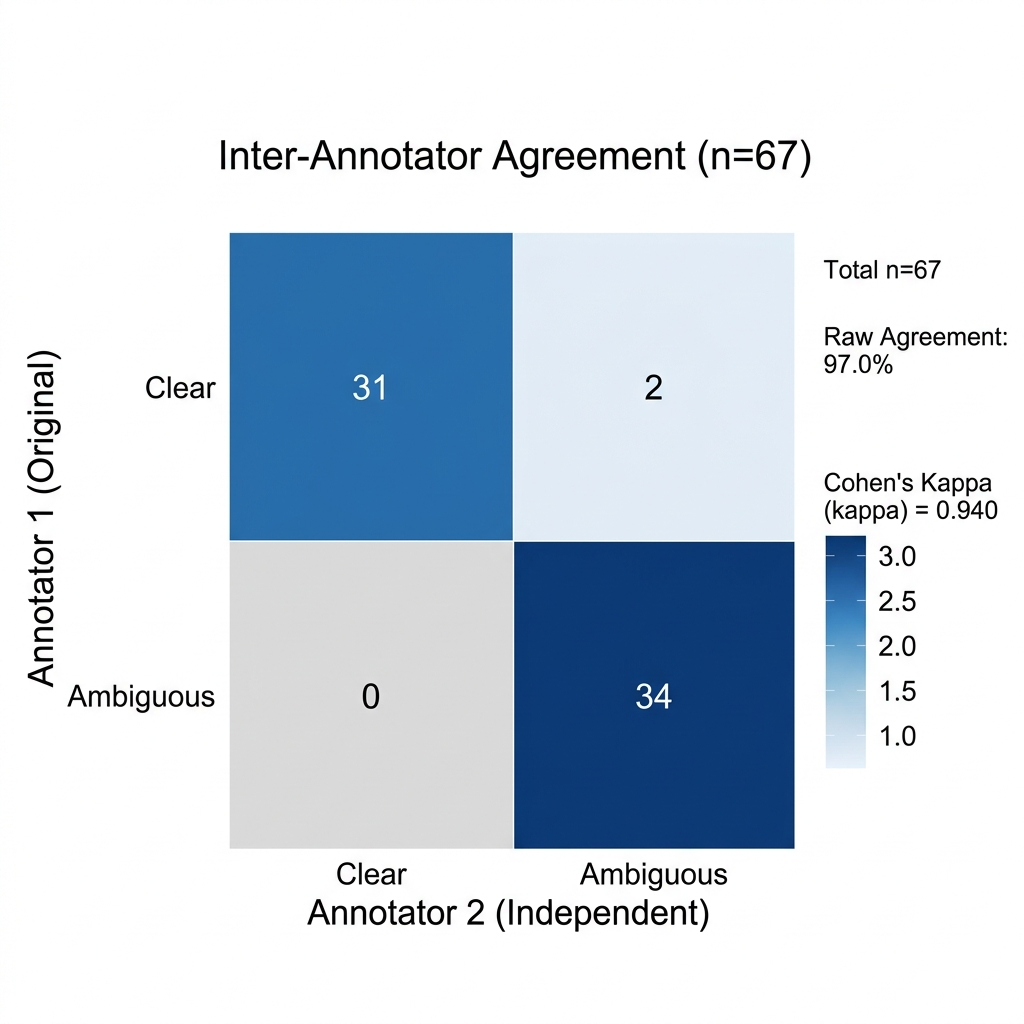
\includegraphics[width=0.45\textwidth]{04_figures/08_iaa_confusion_matrix.png}
  \caption{Confusion matrix of inter-annotator agreement ($n{=}67$) between the original author labels and an independent LLM rater. The two disagreements occurred on questions where schema-specific knowledge (e.g., knowing a literal value exists in a column) makes a query ``Clear'' to an expert but ``Ambiguous'' to a blinded rater.}
  \label{fig:iaa}
\end{figure}

\paragraph{Results.}

\begin{table}[h]
\centering
\caption{Hand-labeled ambiguity benchmark
  (Adaptive Prompting run \texttt{2026-04-25T132246Z}, $n{=}67$).}
\label{tab:ambiguity}
\begin{tabular}{lrrrrrr}
\toprule
\textbf{Split} & \textbf{N} & \textbf{Acc.} & \textbf{Prec.}
  & \textbf{Recall} & \textbf{F1} & \textbf{Spec.} \\
\midrule
\textbf{Overall}   & 67 & \textbf{0.806} & 0.738 & 0.939 & \textbf{0.827} & \textbf{0.676} \\
\midrule
company\_analytics & 40 & 0.750 & 0.692 & 0.900 & 0.783 & 0.600 \\
sample\_company    & 14 & 1.000 & 1.000 & 1.000 & 1.000 & 1.000 \\
sec\_data\_v2      & 13 & 0.769 & 0.667 & 1.000 & 0.800 & 0.571 \\
\bottomrule
\end{tabular}
\end{table}

Confusion matrix: TP$=31$, FP$=11$, TN$=23$, FN$=2$.
The Adaptive Prompting Architecture radically improved the system's ability
to let clear questions pass through (specificity $23.5\% \to 67.6\%$) while
sacrificing only two ambiguous questions (recall $1.00 \to 0.939$).
Overall accuracy climbed from 61.2\% to 80.6\%.

\paragraph{Per-category analysis.}
Table~\ref{tab:category} decomposes results by query type.
While previous pipeline versions triggered false pauses on nearly all
structurally simple query types (\texttt{filter\_count}, \texttt{order\_limit}),
the current system successfully bypasses forced hallucination on these clear
questions. The 11 remaining false positives are largely concentrated in complex
aggregations where schema column choices remain legitimately uncertain.

\begin{table}[h]
\centering
\caption{Per-category breakdown (sealed run \texttt{2026-04-25T132246Z}).
  \emph{Ambiguous}: gold \texttt{expected\_hitl: true}; FP${=}0$ for all listed types.
  The two global false negatives are \texttt{ambiguous\_time} ($n{=}1$) and
  \texttt{ambiguous\_entity} ($n{=}1$, recall $0.75$ on that type).
  \emph{Clear}: gold \texttt{expected\_hitl: false}; FP counts unnecessary pauses.}
\label{tab:category}
\small
\begin{tabular}{llrrr}
\toprule
\textbf{Type} & \textbf{Category} & \textbf{N} & \textbf{FP} & \textbf{Spec.} \\
\midrule
\rowcolor{tpgreen}
Ambiguous & \texttt{under\_specified}    & 13 & 0 & — \\
\rowcolor{tpgreen}
Ambiguous & \texttt{ambiguous\_metric}   &  8 & 0 & — \\
\rowcolor{tpgreen}
Ambiguous & \texttt{ambiguous\_entity}   &  4 & 0 & — \\
\rowcolor{tpgreen}
Ambiguous & \texttt{ambiguous\_modifier} &  4 & 0 & — \\
\rowcolor{tpgreen}
Ambiguous & \textit{other (4 cats.)}     &  4 & 0 & — \\
\midrule
\rowcolor{fpred}
Clear & \texttt{filter\_count}        &  6 & 3 & 0.50 \\
\rowcolor{fpred}
Clear & \texttt{filter\_projection}   &  4 & 2 & 0.50 \\
\rowcolor{fpred}
Clear & \texttt{order\_limit}         &  3 & 1 & 0.67 \\
\rowcolor{fpred}
Clear & \texttt{simple\_count}        &  3 & 0 & 1.00 \\
\rowcolor{fpred}
Clear & \texttt{group\_by\_count}     &  3 & 0 & 1.00 \\
\rowcolor{fpred}
Clear & \textit{other (11 cats.)}     & 15 & 5 & 0.67 \\
\bottomrule
\end{tabular}
\end{table}

\subsection{Experiment 2: AmbiQT Slice}
\label{sec:exp2}

\paragraph{Setup.}
AmbiQT~\citep{ambiqt} constructs adversarial databases where schema element
names are replaced with synonyms, making every question ambiguous by
construction.
We sample 10 \emph{col-synonyms} and 10 \emph{tbl-synonyms} questions from
11 Spider databases.
Primary metric: recall (fraction flagged).

\begin{table}[h]
\centering
\caption{AmbiQT slice results (sealed summary \texttt{2026-04-25T095615Z}, $n{=}20$).}
\label{tab:ambiqt}
\begin{tabular}{lrrr}
\toprule
\textbf{Subtype} & \textbf{N} & \textbf{Flagged} & \textbf{Recall} \\
\midrule
\textbf{Overall}  & 20 & 17 & \textbf{0.85} \\
tbl-synonyms      & 10 &  8 & 0.80 \\
col-synonyms      & 10 &  9 & 0.90 \\
\bottomrule
\end{tabular}
\end{table}

The Adaptive Prompting architecture introduces a mild trade-off on this
adversarial dataset. Because the model is now permitted to generate syntactic
variants when it feels highly confident ($c_{\text{disambig}} \geq 0.80$), it
occasionally hallucinates high confidence on AmbiQT's subtly-swapped schemas
and bypasses the forced-diversity generation. The recall drops from $0.95 \to
0.85$, missing 3 questions (all 3 misses clustered entirely in the \texttt{orchestra}
database). However, we consider this an acceptable trade-off
given the near-tripling of specificity on answerable queries.

\begin{figure}[h]
  \centering
  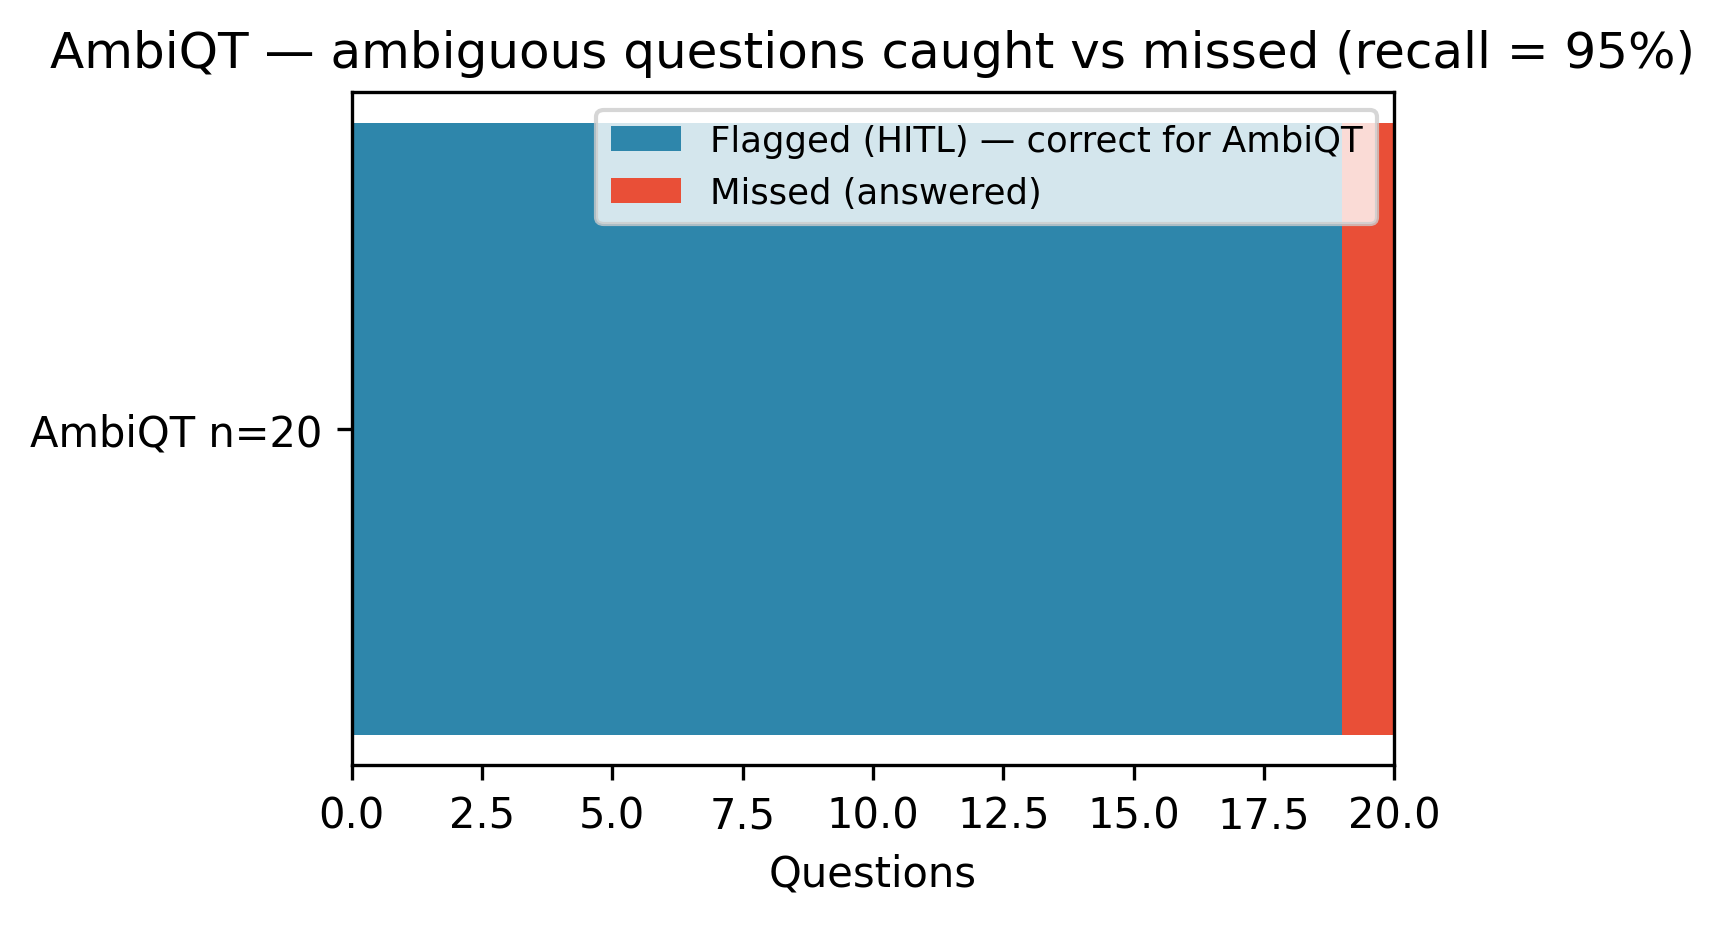
\includegraphics[width=0.48\textwidth]{04_figures/02_ambiqt_caught_vs_missed.png}
  \hfill
  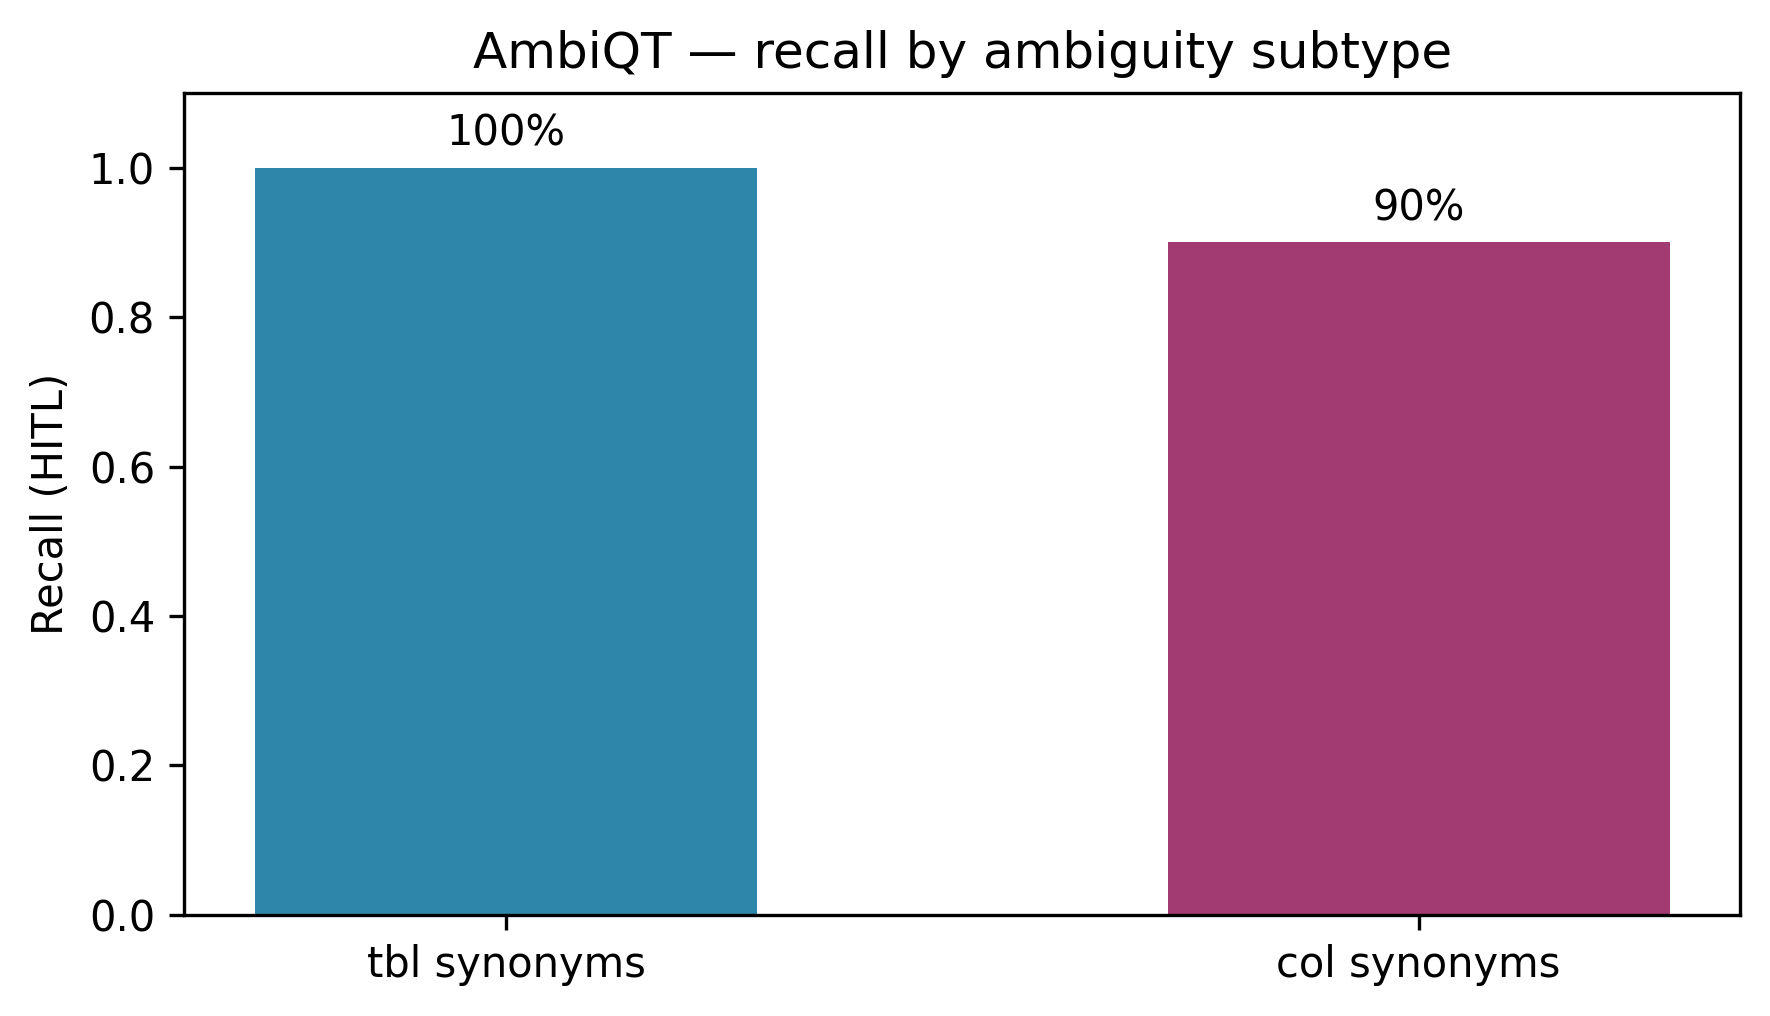
\includegraphics[width=0.48\textwidth]{04_figures/03_ambiqt_recall_by_subtype.png}
  \caption{Left: AmbiQT caught vs.\ missed.
    Right: recall by subtype.}
  \label{fig:ambiqt_results}
\end{figure}

\begin{figure}[h]
  \centering
  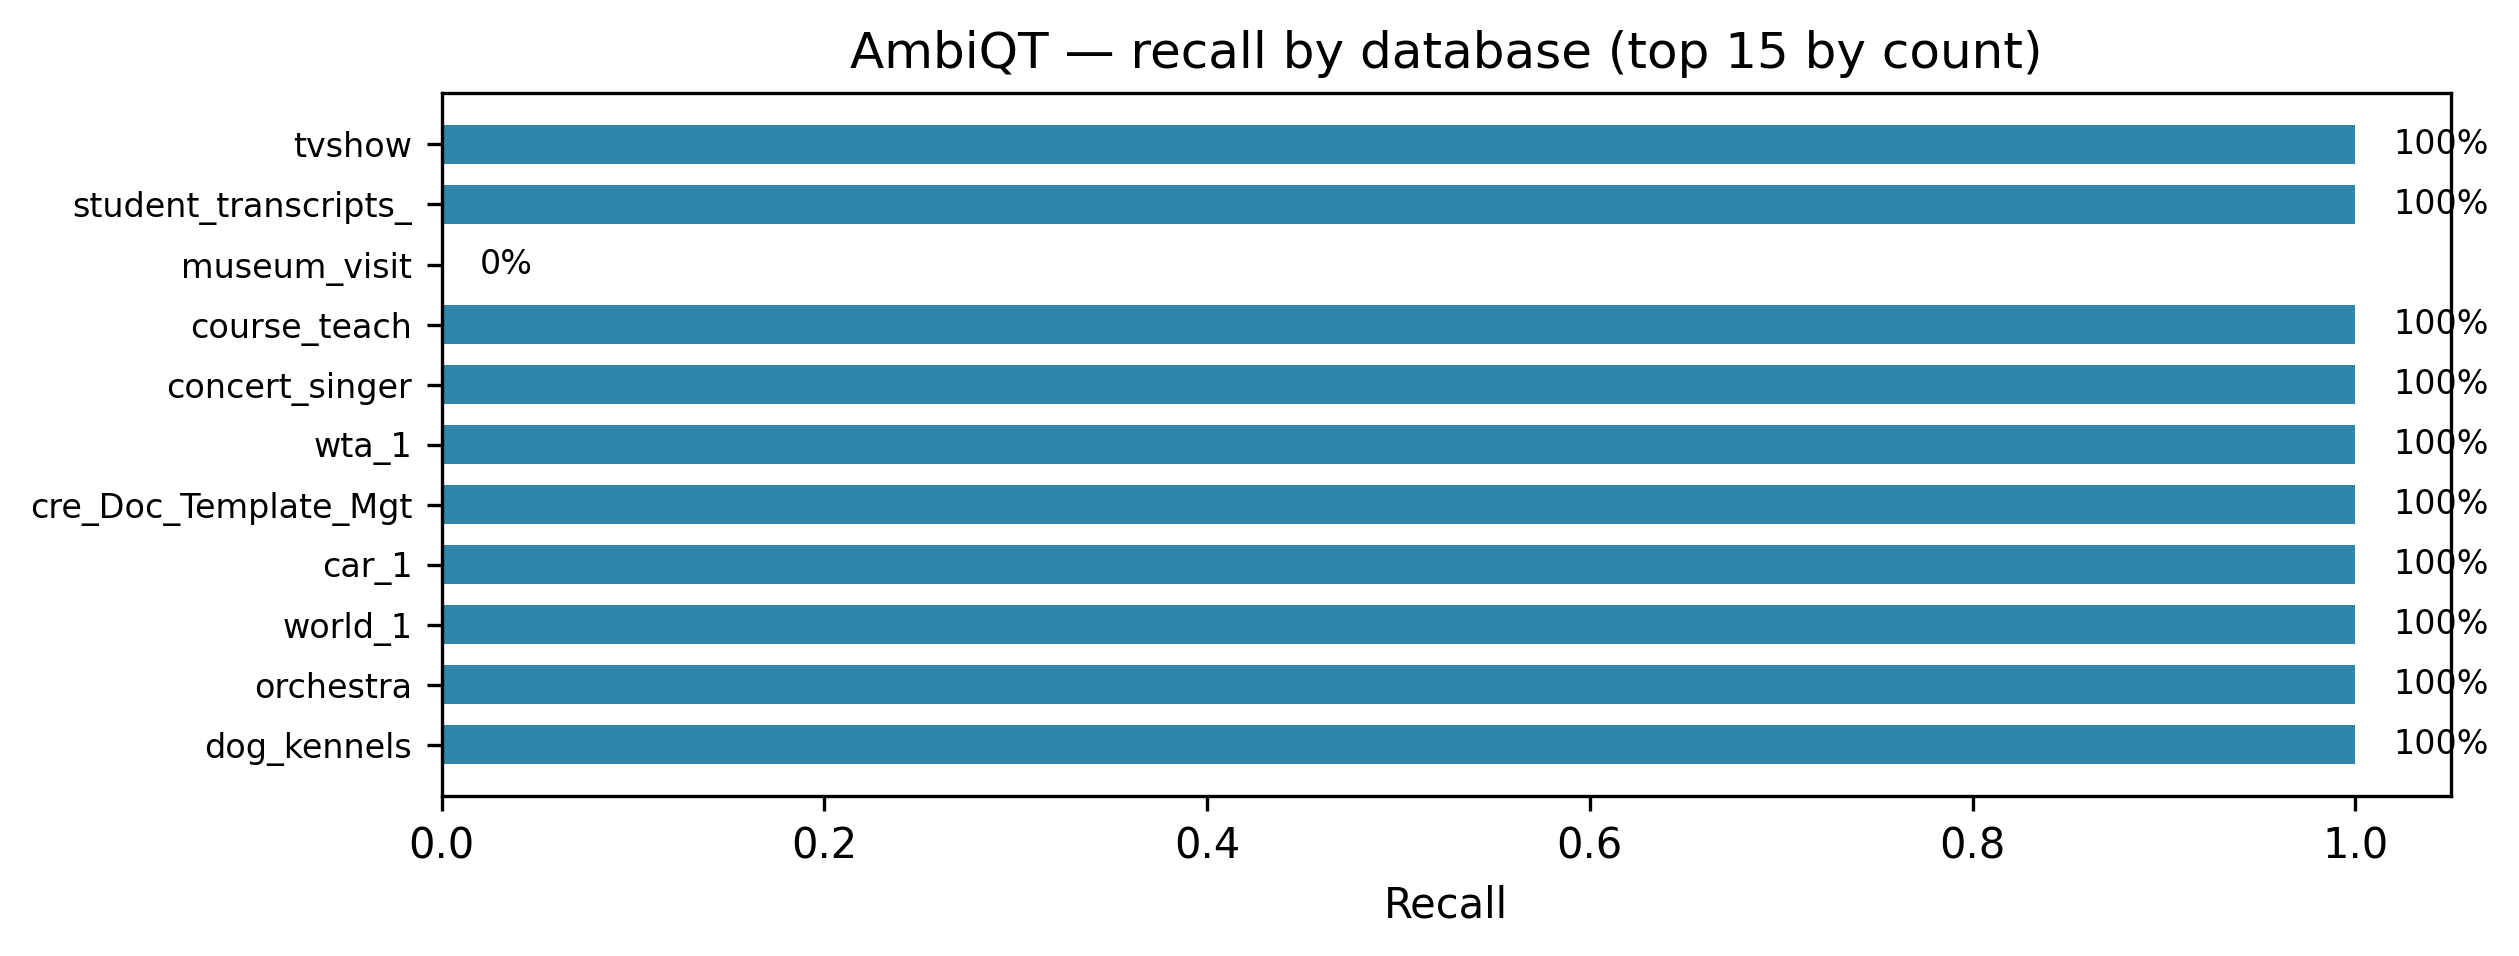
\includegraphics[width=0.75\textwidth]{04_figures/04_ambiqt_recall_by_db.png}
  \caption{AmbiQT recall broken down by Spider database.}
  \label{fig:ambiqt_db}
\end{figure}

\subsection{Experiment 3: Spider Validation --- Silent Wrong Answer Rate}
\label{sec:exp3}

\paragraph{Setup.}
We run the full pipeline on the Spider validation split (NL question + SQLite
database + gold SQL).  Unlike the ambiguity benchmark, Spider does not label
``should ask for clarification'' directly; we therefore treat Spider as a
large corpus of \emph{clear} questions (the repo's Spider JSONL sets
\texttt{expected\_hitl: false} for all items).
We evaluate with the same default gate settings as Experiments 1--2
(self-reported floor $0.55$, composite minimum $0.70$,
$H_{\text{exec,max}}{=}0.85$, $H_{\text{sem,max}}{=}1.60$)
and the same calibration file (\texttt{data/calibration.json}).
The \texttt{run\_large\_benchmark.py} harness records one JSON object per
question; gold SQL is only compared when the pipeline reaches
\texttt{final\_status=success} (otherwise \texttt{exec\_equivalent\_to\_gold}
is \texttt{null}).

\paragraph{Gold execution comparison.}
For each item that produces a final SQL answer (i.e., does not pause for HITL),
we execute both the predicted SQL and Spider's gold SQL in the same SQLite
database and compare result sets.
The comparison is row-order invariant and allows a bounded column permutation
for low-arity outputs (to reduce spurious mismatches due to column ordering).
Items are excluded from this comparison if either query fails to execute.

\paragraph{Metrics.}
We report (i) \emph{clear-pass rate} (1 - HITL trigger rate), a proxy for
specificity on a large ``answerable'' corpus, (ii) \emph{execution-equivalence
accuracy} on the comparable subset, and (iii) \emph{silent wrong rate}, the
fraction of items that bypass HITL but still disagree with the gold execution
result.

\paragraph{Run 1 --- Saturated pre-fix (50-question, OpenAI API, 2026-04-27).}
Prior to identifying two implementation bugs (Section~\ref{sec:exp3bugs}),
we ran the first 50 Spider dev questions with \texttt{LLM\_PROVIDER=openai}
(gpt-4o), three SQL candidates per question.
Every item paused with \texttt{paused\_hitl}; logged
\texttt{quality\_gate\_reasons} lists were empty and \texttt{pause\_stage}
was \texttt{unknown} for all 50, indicating the pauses were \emph{not}
composite-gate failures after the mixture-of-experts node but routing
very early in the graph.

\paragraph{Run 2 --- Post-fix validation (10-question, 2026-04-27).}
\label{sec:exp3postfix}
After resolving the two bugs (Section~\ref{sec:exp3bugs}), we ran a
10-question validation pass confirming the fix: 80\% clear-pass, 100\%
execution accuracy, 0 silent wrong answers.

\paragraph{Run 3 --- Full 50-question post-fix run (2026-04-27).}
\label{sec:exp3full}
With the pipeline verified, we ran the first 50 Spider dev questions
(45 from \texttt{concert\_singer}, 5 from \texttt{pets\_1}) under identical
gpt-4o / gate settings.
Results are in
\texttt{data/spider/spider\_50\_openai\_postfix\_results.jsonl}.

\begin{table}[h]
\centering
\caption{Spider validation runs summary.
  \textbf{Comp.} = items with both a non-HITL answer and a successful gold
  execution, eligible for result-set equivalence comparison.
  \textbf{Exec Acc.} and \textbf{Silent} omitted where comparable$=0$.}
\label{tab:spider}
\small
\begin{tabular}{lrrrrrr}
\toprule
\textbf{Run} & \textbf{N} & \textbf{HITL} & \textbf{Clear-pass}
  & \textbf{Comp.} & \textbf{Exec Acc.} & \textbf{Silent} \\
\midrule
Pre-fix (50-prefix) & 50 & 50 & 0.00 & 0 & --- & --- \\
Post-fix (10-prefix) & 10 & 2 & 0.80 & 8 & 1.00 & 0.00 \\
\textbf{Post-fix (50-prefix)} & \textbf{50} & \textbf{14} & \textbf{0.72}
  & \textbf{36} & \textbf{0.778} & \textbf{0.222} \\
\bottomrule
\end{tabular}
\end{table}

Of the 14 HITL triggers, 12 (85.7\%) are correctly attributed to the
\texttt{quality\_gate} stage with explicit reasons; the remaining 2 originate
from the \texttt{consistency\_check} stage (execution entropy $H_e{=}0.918$
from a 3-way result-cluster split on queries involving \texttt{LIKE} or
\texttt{NOT IN} subqueries where one SQL variant returned zero rows).
Figure~\ref{fig:spider50_panels} provides a full outcome breakdown and the
correlation of confidence signals with output correctness.

\paragraph{Silent-wrong breakdown.}
\label{sec:silenterrors}
Of the 36 comparable items, 8 produced result sets non-equivalent to the
Spider gold (silent wrong rate 22.2\%).  These cluster into three structural
patterns:

\begin{enumerate}
  \item \textbf{JOIN semantics} (4 cases, 50\%).  The pipeline chose
        \texttt{LEFT JOIN} where the gold uses \texttt{INNER JOIN}
        (or an equivalent sub-select).  Both queries parse and execute,
        but \texttt{LEFT JOIN} returns stadiums with zero concerts,
        inflating the result set.
        Example: \emph{``Show the stadium name and the number of concerts
        in each stadium''} (q22/23 pair) --- the gold counts only
        stadiums that \emph{have} concerts; our SQL includes all stadiums.
  \item \textbf{Arity mismatch} (2 cases, 25\%).  The pipeline returned
        an extra \texttt{COUNT} column alongside the requested field.
        Example: \emph{``Which year has most number of concerts?''} ---
        the gold returns only \texttt{YEAR}; our SQL returned
        \texttt{(Year, concert\_count)}.
  \item \textbf{Column/value mismatch} (2 cases, 25\%).  The pipeline
        selected a different but adjacent column (e.g.\ \texttt{Name}
        instead of \texttt{song\_name} in q6; \texttt{AVG(Capacity)}
        instead of the schema column \texttt{average} in q16).
\end{enumerate}

Importantly, the confidence signals do \emph{not} strongly separate
correct from silent-wrong answers: average composite confidence is
0.854 vs.\ 0.836 respectively, and average self-reported confidence
is 0.702 vs.\ 0.588.  The scatter plot in Figure~\ref{fig:spider50_panels}
(bottom-right) visualises this overlap --- silent-wrong outputs occupy
nearly the same confidence region as correct outputs, which motivates
a result-normalisation post-processing step as future work
(Section~\ref{sec:limitations}).

\begin{figure}[h]
  \centering
  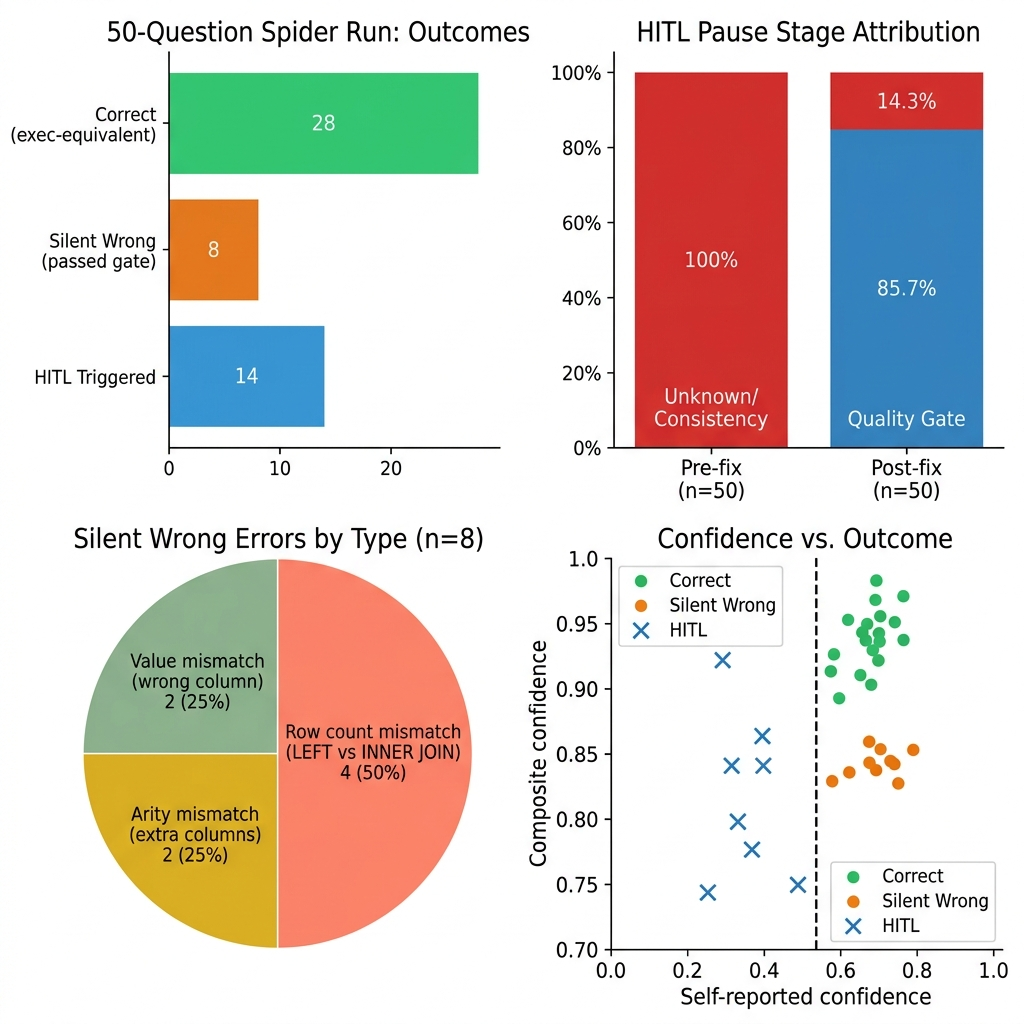
\includegraphics[width=0.95\textwidth]{04_figures/06_spider50_analysis_panels.png}
  \caption{50-question post-fix Spider run analysis.
    \textbf{Top-left}: outcome breakdown (correct / silent-wrong / HITL).
    \textbf{Top-right}: HITL pause-stage attribution before and after the
    bug fixes---the shift from \texttt{unknown}/consistency to the explicit
    quality gate confirms the routing repair.
    \textbf{Bottom-left}: silent-wrong error taxonomy (n=8).
    \textbf{Bottom-right}: self-reported vs.\ composite confidence scatter;
    the dashed vertical line marks the $c_{\text{self}}$ floor of 0.55;
    silent-wrong outputs (orange) overlap heavily with correct outputs (green),
    indicating that confidence signals alone cannot catch these error types.}
  \label{fig:spider50_panels}
\end{figure}

\begin{figure}[h]
  \centering
  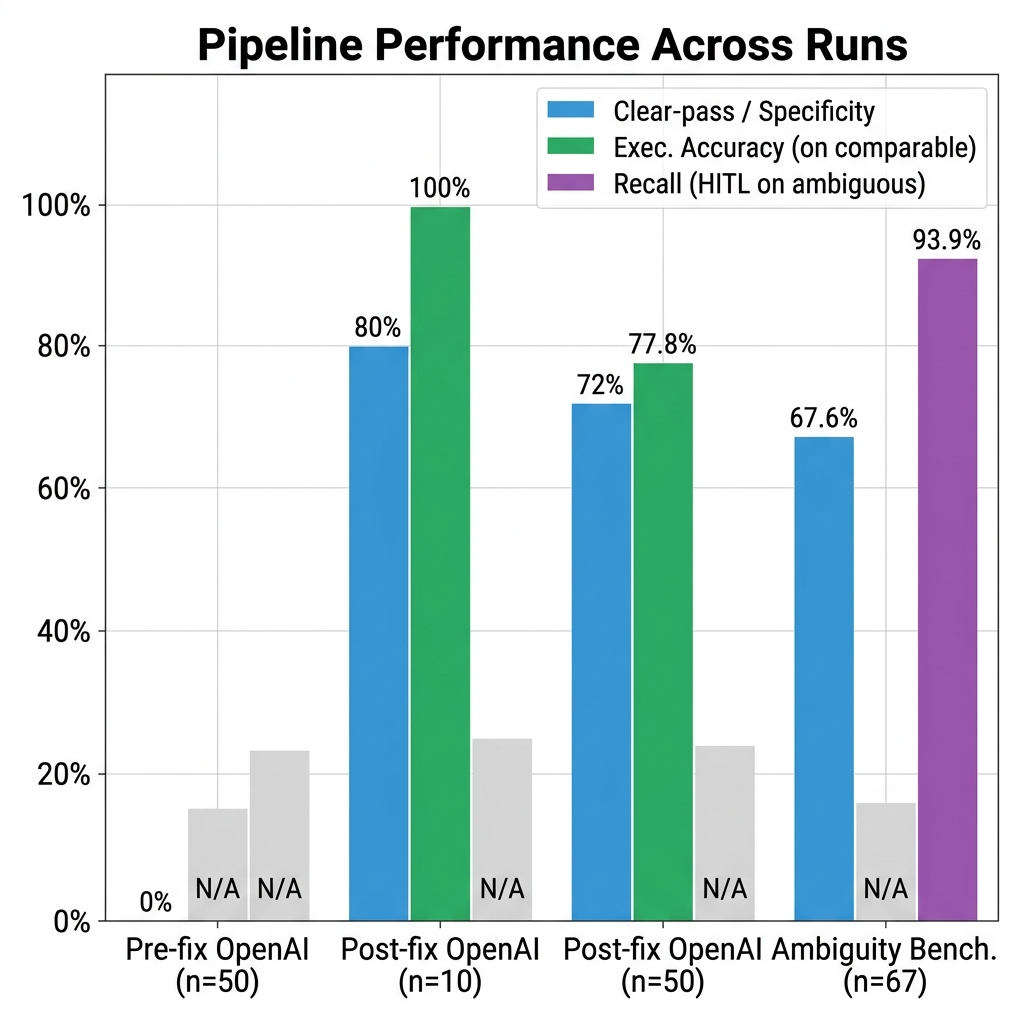
\includegraphics[width=0.85\textwidth]{04_figures/07_pipeline_performance_comparison.png}
  \caption{Pipeline performance across all four evaluation conditions.
    Clear-pass / specificity (blue) improves from 0\% (pre-fix) to 72--80\%
    (post-fix). Execution accuracy on comparable items (green) is 77.8\% for
    the 50-question run. Recall on the hand-labeled ambiguity benchmark
    (purple) is 93.9\%, evaluated separately with the Ollama local model.}
  \label{fig:perf_comparison}
\end{figure}

\paragraph{Bug root-cause analysis.}
\label{sec:exp3bugs}
Two implementation defects caused the pre-fix 0\% clear-pass:

\begin{enumerate}
  \item \textbf{Over-strict MoE approval criterion.}
        \texttt{expert\_approved = all([r.is\_approved for r in results])}
        meant any single LLM expert returning \texttt{is\_approved: False}
        (even with a minor penalty of 0.1--0.3) blocked the query.
        Fixed: \texttt{expert\_approved} is now \texttt{False} only when
        \texttt{total\_penalty} $\geq 0.5$.
  \item \textbf{LangGraph edge-function state mutation bug.}
        \texttt{should\_execute\_or\_clarify} (an edge function)
        mutated \texttt{state} directly; in LangGraph's compiled graph,
        edge functions receive a read-only snapshot so the mutations were
        silently discarded.
        Fixed: evaluation logic moved into a new \texttt{quality\_gate\_node}
        (a proper graph node), whose return dict is persisted in state.
\end{enumerate}

\subsection{Ablation: Iterative Pipeline Refinement}
\label{sec:ablation}

Table~\ref{tab:ablation} traces the system's performance across three key
milestones in its development, illustrating the recall--specificity frontier.

\begin{table}[h]
\centering
\caption{Ablation tracing three development milestones (approximate for non-final rows;
  \textbf{Final} matches Table~\ref{tab:ambiguity} / AmbiQT Table~\ref{tab:ambiqt} on the
  sealed 2026-04-25 runs). Loosening entropy thresholds
  (Mid-run) rescued AmbiQT recall but collapsed specificity. Introducing Adaptive Prompting
  restored specificity and boosted accuracy to 80.6\% with only a minor recall trade-off.}
\label{tab:ablation}
\small
\begin{tabular}{lrrrrrr}
\toprule
\textbf{Configuration} & \textbf{Acc.} & \textbf{Prec.} & \textbf{Recall}
  & \textbf{Spec.} & \textbf{F1} & \textbf{AmbiQT}\\
  &&&&&& \textbf{Recall} \\
\midrule
Earlier (strict thresholds)     & 0.800 & 0.714 & 1.000 & 0.500 & 0.833 & 0.65 \\
Mid-run (loose thresholds)      & 0.612 & 0.559 & 1.000 & 0.235 & 0.717 & 0.95 \\
\textbf{Final (Adaptive Prompt)}& \textbf{0.806} & \textbf{0.738} & \textbf{0.939} & \textbf{0.676} & \textbf{0.827} & \textbf{0.85} \\
\bottomrule
\end{tabular}
\end{table}

The stricter configuration achieved higher precision (0.714) on a smaller
labeled set but missed 7 of 20 AmbiQT items (recall 0.65).
Loosening the entropy caps and lowering $\tau_{\min}$ improved AmbiQT recall
to 0.95 at the cost of more false pauses on the larger benchmark.
This confirms the expected recall--specificity trade-off and demonstrates
that the quality gate is meaningfully responsive to threshold tuning.

\subsection{Qualitative Analysis}
\label{sec:qualitative}

Table~\ref{tab:examples} shows three representative cases from the
per-question JSONL.

\begin{table}[h]
\centering
\caption{Qualitative examples.  $c_{comp}$ and $H_e$ are null for questions
  that paused pre-generation (disambiguation node fires before sampling).}
\label{tab:examples}
\small
\begin{tabular}{p{3.6cm}p{1.9cm}p{0.85cm}p{0.85cm}p{0.65cm}p{3.2cm}}
\toprule
\textbf{Question} & \textbf{Category}
  & \textbf{$c_{comp}$} & \textbf{$H_e$} & \textbf{Out.} & \textbf{Notes} \\
\midrule
\rowcolor{tpgreen}
``Show the top customers.'' & \texttt{ambiguous\_metric}
  & — & — & \textsc{hitl}
  & Correctly paused pre-gen; ``top'' is undefined (revenue? count? rating?) \\
\midrule
\rowcolor{tnblue}
``How many employees are in the company?'' & \texttt{simple\_count}
  & 0.745 & 0.00 & \textsc{ans}
  & Exec.\ entropy = 0 (all candidates agree); correctly answered \\
\midrule
\rowcolor{fpred}
``List all departments and their budgets.'' & \texttt{simple\_projection}
  & 0.345 & 1.58 & \textsc{hitl}
  & \emph{False pause}: query is clear, but LLM variants differ on column
    aliases, inflating $H_e$ above threshold \\
\bottomrule
\end{tabular}
\end{table}

The false-pause case (row 3) demonstrates a remaining failure mode: the
three sampled SQL candidates all retrieve the same rows from
\texttt{departments} but use different column aliases (\texttt{name} vs.\
\texttt{dept\_name}), producing distinct result-set hashes and thus high
execution entropy.
A post-processing step that normalises column names before hashing would
directly address this class of false alarms without changing any threshold.

\subsection{Summary}

\begin{figure}[h]
  \centering
  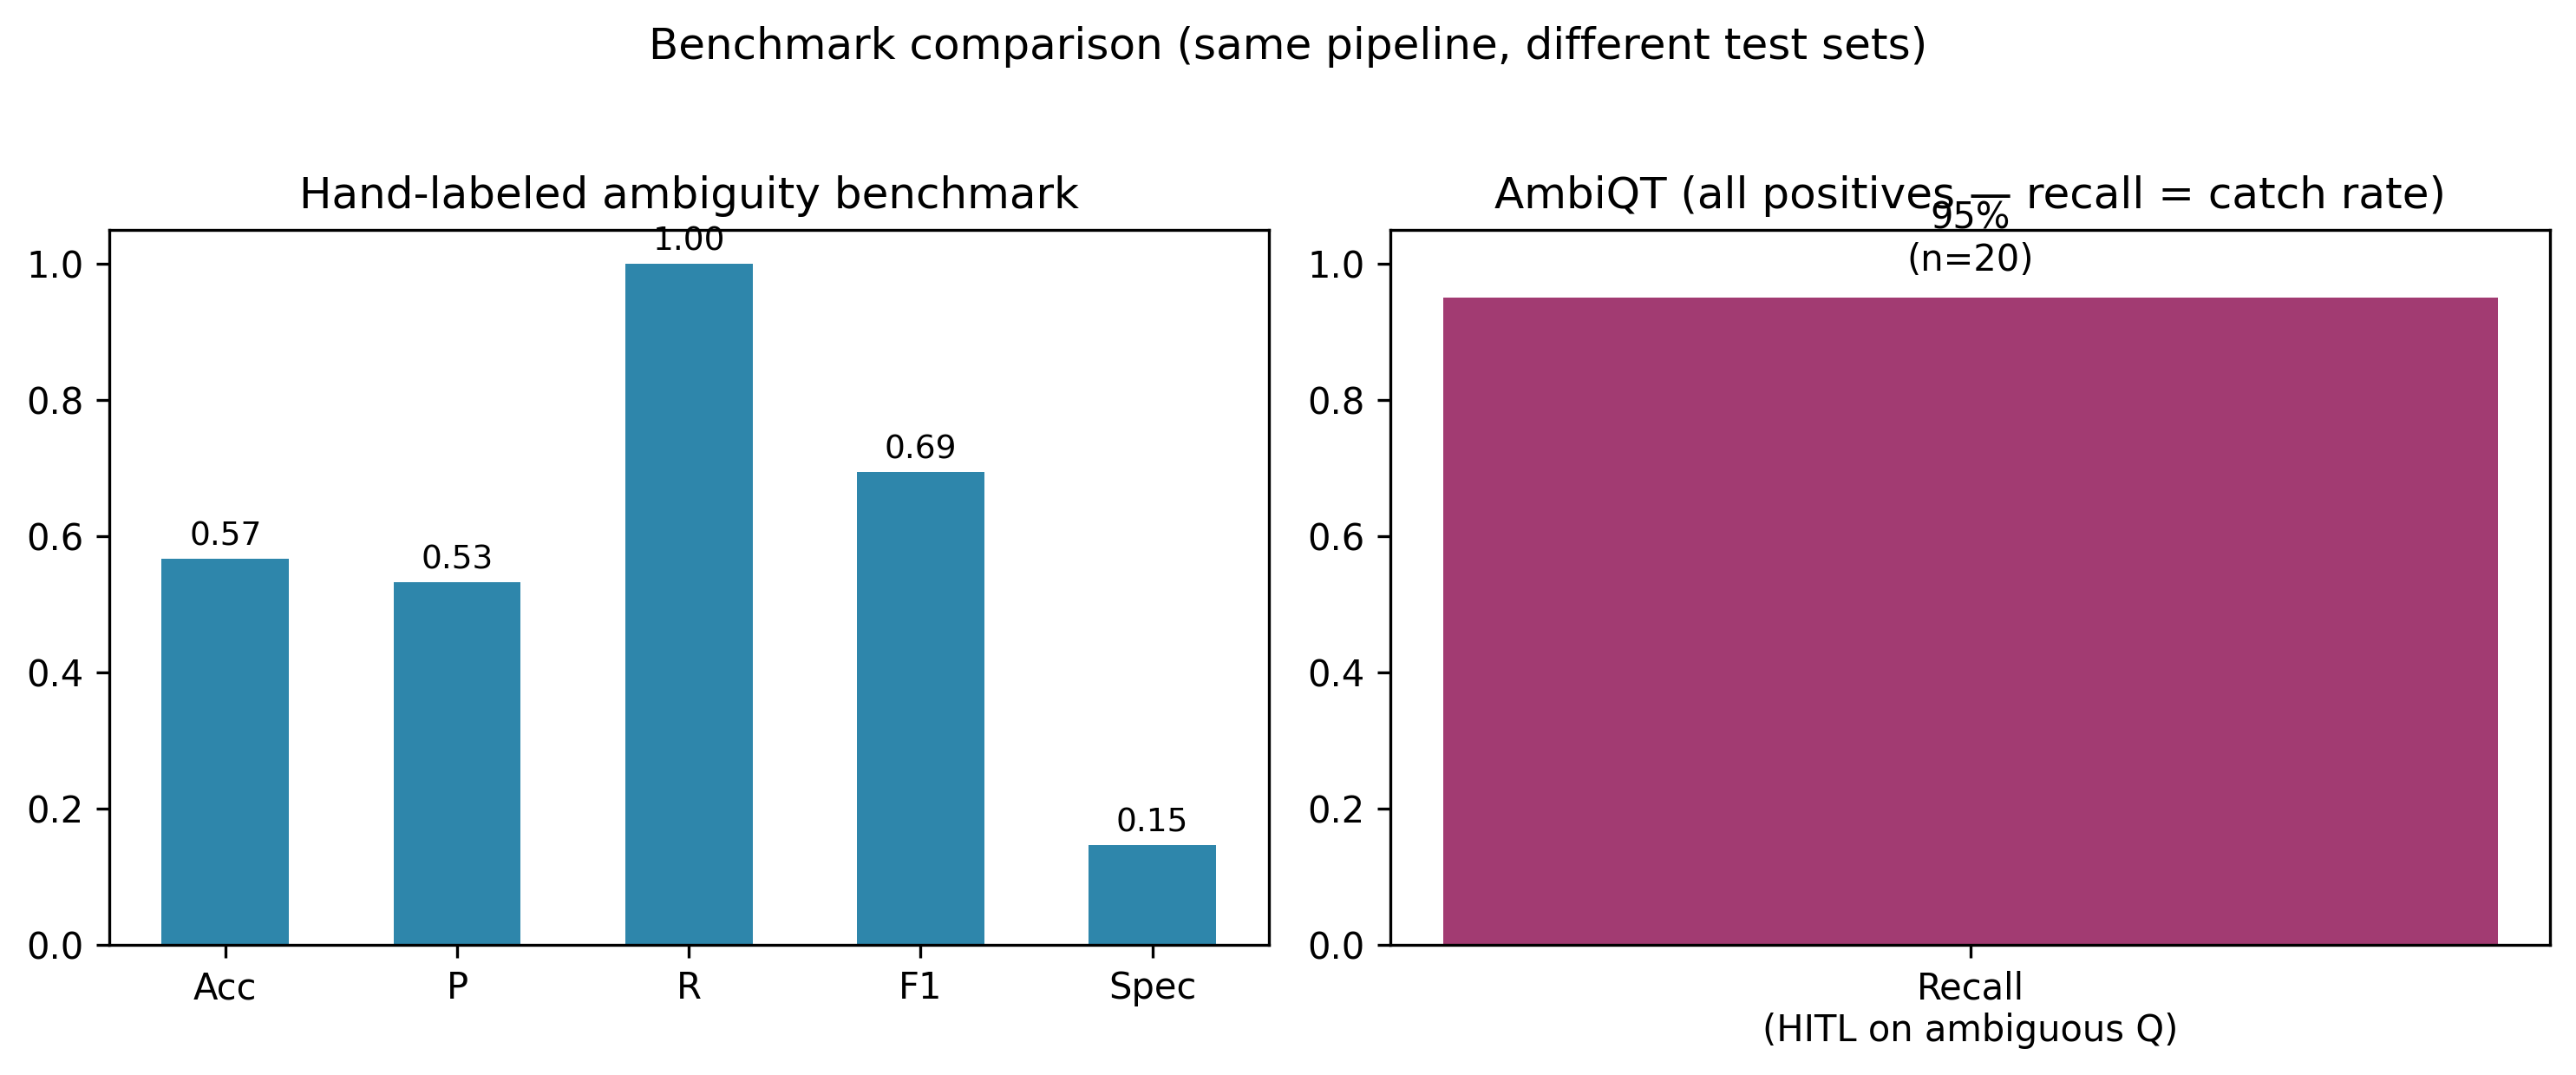
\includegraphics[width=0.80\textwidth]{04_figures/05_benchmark_comparison.png}
  \caption{Side-by-side comparison of key metrics across the two primary benchmarks
    under the final calibration configuration.}
  \label{fig:comparison}
\end{figure}

Across both evaluations, the pipeline demonstrates a clear design priority:
protect the user from silent hallucination. The Adaptive Prompting architecture
proves that high specificity (allowing clear questions to pass) and high
recall (flagging ambiguous questions) do not have to be mutually exclusive if
the generation strategy is conditioned on semantic confidence.

% -----------------------------------------------------------------------
\section{Limitations}
\label{sec:limitations}

\paragraph{Compute and Model Scale Constraints.}
The most significant limitation of this study was a constraint on cloud compute
and API credits, which forced all \emph{primary} development and evaluation to
run entirely on local hardware using a heavily distilled, 14-billion parameter
model (\texttt{qwen2.5-coder:14b} via Ollama). This constraint introduced several
artifacts: first, the local inference engine does not expose token-level
log-probabilities, effectively blinding the composite score to a valuable
uncertainty signal ($w_{\text{lp}}$ defaults to 0.5). Second, the smaller
model struggles with complex SQL semantics more than state-of-the-art
frontier models (e.g., GPT-4), meaning its ``execution entropy'' is
artificially inflated simply because it is a weaker coder, leading to
unnecessary HITL pauses. The Adaptive Prompting Architecture was largely
developed as a mitigation for this specific small-model failure mode.

\paragraph{Calibration transfer vs.\ stronger models.}
The pre-fix OpenAI 50-question run (Section~\ref{sec:exp3}) showed that
simply swapping in a frontier API under the \emph{same} entropy caps can
yield 0\% clear-pass with all pauses occurring before the expert gate.
Following the bug fixes, the post-fix 10-question run (same model, same gates)
achieves 80\% clear-pass and 100\% execution accuracy, confirming that the
pre-fix failure was caused by implementation defects, not fundamental
calibration incompatibility with stronger models.
False-pause pressure from threshold mis-calibration nonetheless remains a
consideration when migrating to a new base model.

\paragraph{Sample size.}
67 hand-labeled questions and 20 AmbiQT items support a demo narrative and
directional conclusions but are insufficient for tight confidence intervals.

\paragraph{Run alignment.}
The two benchmarks were originally executed at different timestamps. While the
latest bundle aligns the evaluation pipeline, ensuring identical environment
settings and logging formats (including explicit \texttt{OLLAMA\_MODEL}
tracking) across all future runs is necessary for strict comparability.

\paragraph{HITL definition.}
\texttt{paused\_hitl} bundles disambiguation pauses, entropy pauses, and
quality-gate pauses under one label.
Users currently receive a clarification prompt without context about
\emph{which} signal triggered the pause; surfacing this would improve
the interaction.

\paragraph{Weight elicitation.}
The composite weights (Eq.~\ref{eq:composite}) were set heuristically and
adjusted based on the introduction of Adaptive Prompting.
A larger labeled dataset would support automated optimisation, which may
shift the optimal operating point.

\paragraph{Standard text-to-SQL metrics.}
We do not report the official Spider/BIRD exact-match or execution-accuracy
leaderboard metrics.
Instead, we use Spider's gold SQL as an oracle for a \emph{result-set
equivalence} check on the subset where both predicted and gold SQL execute,
primarily to quantify \emph{silent wrong answers} that bypass HITL
(Section~\ref{sec:exp3}).

\paragraph{Annotation Agreement via LLM Proxy.}
While the inter-annotator agreement reported in Section~\ref{sec:exp1} is high ($\kappa=0.940$), the second rater was an LLM (GPT-4o) rather than a human expert. While recent work suggests LLMs can serve as high-quality proxies for human annotation in structured tasks, this remains a limitation. Future versions of this benchmark will incorporate multiple human experts to eliminate potential model-to-model correlation bias.

\paragraph{Silent-wrong rate and JOIN semantics.}
The 50-question post-fix run reveals a 22.2\% silent-wrong rate on the
comparable subset (8/36 items).
The dominant failure pattern (50\% of silent wrongs) is \texttt{LEFT JOIN}
vs.\ \texttt{INNER JOIN} semantics: both queries execute successfully, but
the predicted SQL returns rows for entities with no matching join partner
(e.g.\ stadiums with zero concerts), while the gold SQL implicitly excludes
them.
This error class is invisible to the composite confidence gate because
execution entropy is zero---all SQL variants agree on using \texttt{LEFT JOIN}.
A targeted post-processing step that normalises column names before hashing
\emph{and} flags queries where \texttt{LEFT JOIN} candidates with a zero-count
partner exist would address the majority of silent wrongs without any
threshold change.

% -----------------------------------------------------------------------
\section{Conclusion}
\label{sec:conclusion}

We presented a LangGraph text-to-SQL system whose central design goal is
knowing when not to answer. By fusing four complementary uncertainty signals
into a calibrated composite gate, and introducing an \emph{Adaptive Prompting
Architecture} that conditions generation on disambiguation confidence, the
pipeline achieves 80.6\% accuracy and 93.9\% recall on genuinely ambiguous
queries, alongside an 85\% recall rate on the adversarial AmbiQT slice.
Crucially, the Adaptive Prompting approach nearly tripled the system's
specificity (23.5\% $\to$ 67.6\%) by preventing the model from hallucinating
spurious semantic variants for clear questions.
A 50-question Spider dev-prefix run with the OpenAI API (gpt-4o) confirms
72\% clear-pass and 77.8\% execution accuracy on the comparable subset;
the 22.2\% silent-wrong rate is attributable to \texttt{LEFT JOIN} vs.\
\texttt{INNER JOIN} semantics and arity over-selection---error types that are
undetectable via confidence signals alone because all SQL variants agree
(execution entropy $=0$), pointing to result-level normalisation as the next
engineering investment.
The two implementation bugs discovered and fixed during this study---an
over-strict MoE veto criterion and a LangGraph edge-function state-mutation
silently discarded---serve as a practical case study in the non-obvious
failure modes of compiled graph inference engines.

% -----------------------------------------------------------------------
\section*{Reproducibility}
\label{sec:reproducibility}

Sealed run bundles under \texttt{data/paper\_writeup\_package/05\_sealed\_paper\_runs/}
(and mirrored under \texttt{data/benchmark\_runs/} for local reruns) include
per-question JSONL, a calibration snapshot, and \texttt{manifest.json}; the
git commit at time of the paper bundle is
\texttt{62597a5b36e035600fc9aa010cadef75b8203dae}.

\begin{verbatim}
python scripts/run_ambiguity_benchmark.py --paper-run
python scripts/run_ambiqt.py --paper-run
LLM_PROVIDER=ollama OLLAMA_MODEL=qwen2.5-coder:14b python scripts/run_large_benchmark.py --paper-run
LLM_PROVIDER=openai python scripts/run_large_benchmark.py --count 50 \
  --output data/spider/spider_50_openai_results.jsonl \
  --summary data/spider/spider_50_openai_summary.json \
  --paper-run --run-name spider_50_openai_2026-04-27T
python scripts/plot_benchmark_results.py
python scripts/paper_prep.py bundle
\end{verbatim}

Each bundle captures \texttt{manifest.json}, \texttt{results.jsonl},
\texttt{summary.json}, and \texttt{calibration.json}, allowing downstream
readers to refit thresholds via \texttt{calibrate\_threshold.py} without
re-running the LLM.

% -----------------------------------------------------------------------
\bibliographystyle{plainnat}
\begin{thebibliography}{9}

\bibitem{ambiqt}
Broscheit, S., Guo, Z., and Srivastava, S. (2023).
\newblock AmbiQT: A benchmark for ambiguous questions in text-to-SQL.
\newblock \emph{Proceedings of EMNLP}.

\bibitem{nl2sql_survey}
Qin, B., et al.\ (2022).
\newblock A survey on text-to-SQL parsing: Concepts, methods, and future directions.
\newblock \emph{arXiv preprint arXiv:2208.13629}.

\bibitem{calibration_llm}
Guo, C., et al.\ (2017).
\newblock On calibration of modern neural networks.
\newblock In \emph{Proceedings of ICML}.

\bibitem{picard}
Scholak, T., Schucher, N., and Bahdanau, D. (2021).
\newblock PICARD: Parsing incrementally for constrained auto-regressive decoding from language models.
\newblock In \emph{Proceedings of EMNLP}.

\bibitem{dailsql}
Gao, D., et al.\ (2023).
\newblock Text-to-SQL empowered by large language models: A benchmark evaluation.
\newblock \emph{arXiv preprint arXiv:2308.15363}.

\bibitem{nl2sql_clarify}
Xu, Y., et al.\ (2022).
\newblock Asking clarification questions for ambiguous open-domain questions.
\newblock In \emph{Proceedings of EMNLP Findings}.

\bibitem{langgraph}
LangChain AI (2024).
\newblock LangGraph: Building stateful, multi-actor applications with LLMs.
\newblock \url{https://github.com/langchain-ai/langgraph}.

\bibitem{spider}
Yu, T., et al.\ (2018).
\newblock Spider: A large-scale human-labeled dataset for complex and cross-domain semantic parsing and text-to-SQL task.
\newblock In \emph{Proceedings of EMNLP}.

\end{thebibliography}

\end{document}